
\chapter{Cache evaluation analysis}

\section{Payloads}

\subsection{Zephyr based matrix-multiplication}

% TODO: is zephyr even imporant here? idk
Matrix multiplication is a fundamental operation in many scientific and engineering applications, including high-performance computing (e.g., finite element methods), machine
learning (e.g., linear algebra), and edge computing (e.g., DSP, edge-AI, cryptography), among others. This section discusses the implementation and of various cache multiplication algorithms,
taking into the account cache usage in each of them.

The algorithms have been implemented using the Zephyr RTOS as the execution platform. This particular RTOS has been chosen due to its support for a wide range of hardware boards,
its user-friendly build system (\texttt{CMake} alongside the \texttt{west} helper), its use of the C programming language, and its robust real-time capabilities.
Moreover, Zephyr is a collaborative project with the Linux Foundation and is the fastest-growing real-time operating system \cite{zephyrlotsofcommits}. It has commercial support
from major vendors in the embedded and edge computing sectors, such as Nordic Semiconductors, NXP, STMicroelectronics, Microchip, and many others \cite{aboutzephyr}. Additionally,
it is backed by major companies in the technology sector, including, among others, Google, Meta, Qualcomm and Intel \cite{zephyrmetagoogle, zephyrmembers}.

\noindent This payload will be used for testing \textit{different software configurations}, while the simulated \textit{hardware remains unchanged}.

\subsubsection*{Naive approach}
The naive approach to matrix multiplication involves three nested loops iterating over the rows and columns of the matrices. This method, is called naive, as it is simple, but not cache-friendly
due to its poor data locality.

\begin{center}
	\centering
	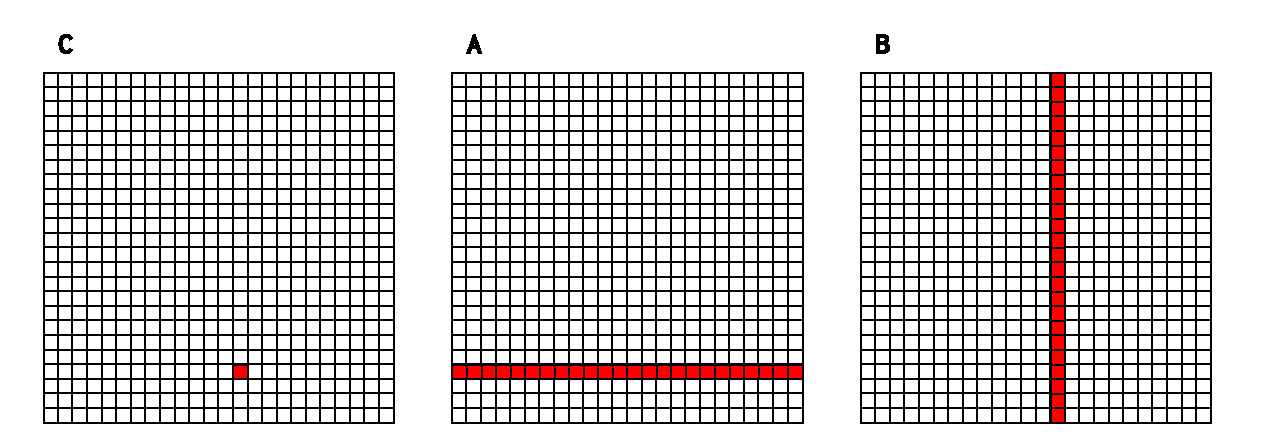
\includegraphics[width=0.75\textwidth]{figures/05-analysis/mm_naive.pdf}
	\captionof{figure}{Visual representation of the multiplication using the naive approach}
	\label{fig:mm_naive}
\end{center}

The naive approach involves three nested loops, iterating over the rows columns of the matrices:

\begin{center}
\centering
\begin{minipage}{\linewidth}
\begin{lstlisting}[
	style=lstC,
    caption={Naive matrix multiplication implemented in C programming language}
    ]
for (i = 0; i < SIZE; i++) {
	for (j = 0; j < SIZE; j++) {
		for (k = 0; k < SIZE; k++) {
			c[i * SIZE + j] += a[i * SIZE + k] * b[k * SIZE + j];
		}
	}
}
\end{lstlisting}
\end{minipage}
\end{center}

\noindent If the matrices are represented as a 1D array in memory, the naive approach to matrix multiplication results in poor cache performance due to suboptimal data locality.
The naive algorithm frequently jumps between distant memory locations, leading to cache misses.

\subsubsection*{Block based approach}
The block-based approach improves cache performance by dividing the matrices into smaller sub-matrices (blocks) that fit into the cache.

\begin{center}
	\centering
	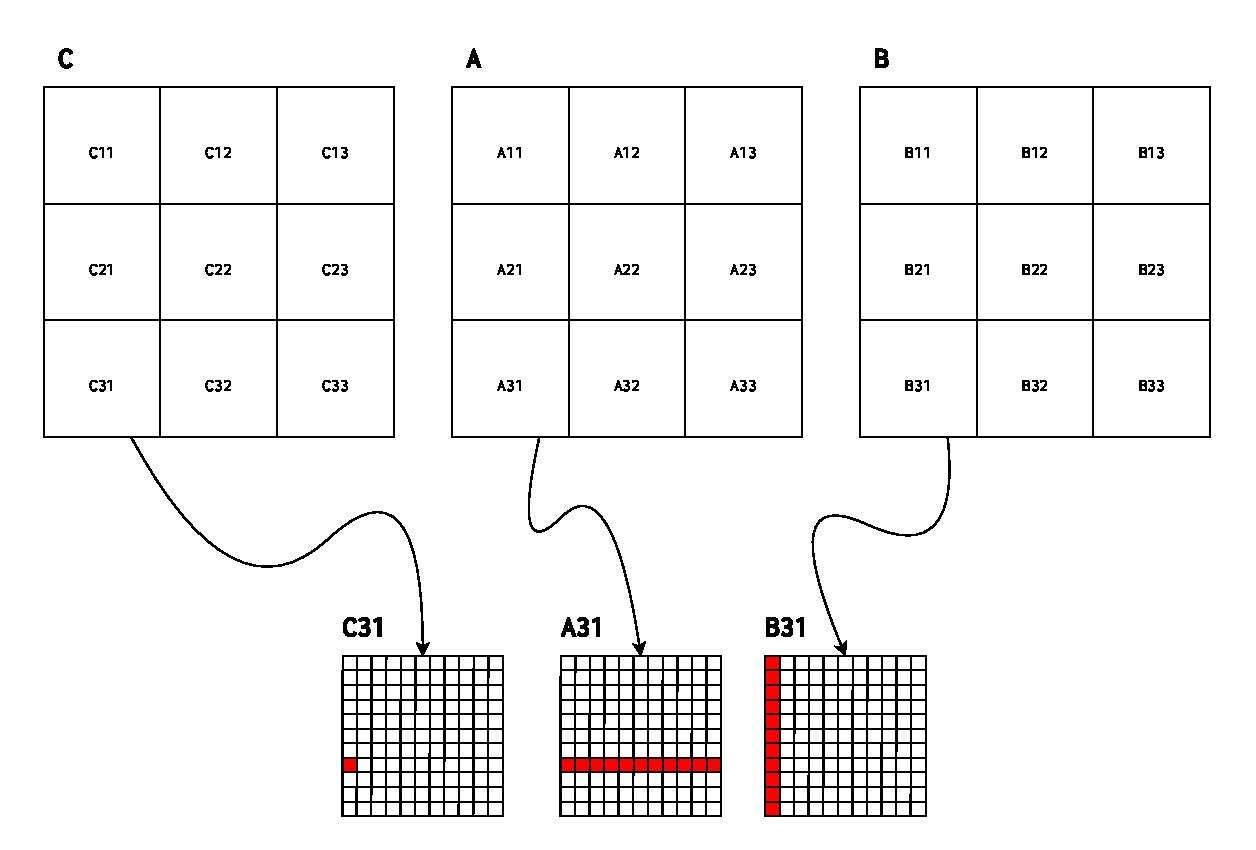
\includegraphics[width=0.75\textwidth]{figures/05-analysis/mm_block.pdf}
	\captionof{figure}{Visual representation of the multiplication using the block based approach}
	\label{fig:mm_block}
\end{center}

\noindent By dividing the large matrix into smaller matrices, data locality is significantly improved, reducing the number of cache misses. This method is particularly effective for
large matrices, where the naive approach would otherwise result in frequent cache evictions. The larger blocks (A11, A12, B11, B12, etc.) are then multiplied and added together.
Selecting the optimal block size is a trade-off. The block size should be small enough to allow the data to fit into the cache but as large as possible to minimize runtime
overhead. Decreasing the block size results in increased runtime overhead because more instructions need to be executed.

\noindent The block-based algorithm has been implemented as follows:
\begin{center}
\centering
\begin{minipage}{\linewidth}
\begin{lstlisting}[
	style=lstC,
    caption={Block based matrix multiplication in C programming language}
    ]
const int B = BLOCK_SIZE;
for (i = 0; i < SIZE; i += B) {
	for (j = 0; j < SIZE; j += B) {
		for (k = 0; k < SIZE; k += B) {
			/* B x B mini matrix multiplications */
			for (i1 = i; i1 < i + B && i1 < SIZE; i1++) {
				for (j1 = j; j1 < j + B && j1 < SIZE; j1++) {
					for (k1 = k; k1 < k + B && k1 < SIZE; k1++) {
						c[i1 * SIZE + j1] += a[i1 * SIZE + k1] * b[k1 * SIZE + j1];
					}
				}
			}
		}
	}
}
\end{lstlisting}
\end{minipage}
\end{center}

\subsection{Linux kernel}
% TODO: this section is a biiit short
The Linux kernel is a core component of many devices, ranging from relatively small microcontrollers, to desktop computers and even HPC clusters.
It has been selected as a payload due to its relatively lengthy and memory-access-intensive boot process, such as during the unpacking of initramfs. This process is
characterized by a mix of sequential and random memory access patterns, providing a good benchmark for testing various cache configurations.

\noindent This payload will be used for testing \textit{different hardware configurations}, while the \textit{software remains unchanged}.

\section{Cache model verification}

\subsection{Verification against QEMU TCG Cache Modeling plugin}
The cache model was also verified against the QEMU TCG Cache Modeling plugin, introduced in section (\ref{sec:qemu_cache}).
Since this cache model is only supported for virtual QEMU platforms, it was necessary to find a platform that is compatible with both QEMU and Renode - the simulator that generates
the trace files for the model created in this work.

The RISC-V-based SiFive HiFive1 Rev B (\texttt{fu310} SoC with one \texttt{e31} RV32IMAC core) platform has been selected. This platform meets the necessary requirements for
compatibility with both QEMU and Renode, provides extensive documentation including cache parameters, and features built-in hardware performance counters that will be used in
(\ref{sec:hpc}). The payload against which we will be verifying the cache model results is the Zephyr RTOS-based matrix multiplication algorithm (naive approach). Due to the
platform's limited RAM size, the benchmark sample had to be limited to a matrix of size 16 by 16\footnote{Matrices of size $32^2$ resulted in a stack crash (manifesting itself in
a \textit{Load access fault} exception), while sizes $64^2$ and above resulted in a linker failure due to overflowing memory regions.}. The cache configuration for the \texttt{e31}
core includes a 16 KiB 2-way set-associative instruction cache with a 32-byte block line size with \textit{random} eviction policy and no data cache \cite{fe310docs}.

\noindent The QEMU was invoked with the following parameters:
\begin{verbatim}
qemu-system-riscv32 -nographic           \
	-machine sifive_e                       \ # simulate fu310 SoC
	-icount align=off,sleep=off             \ # decouple virtual and host time
	-kernel payload.elf                     \ # payload executable
	-plugin ./contrib/plugins/libcache.so,  \ # use TCG Cache modelling plugin
	        icachesize=16384,               \ # 16 KiB cache size
	        iassoc=2,                       \ # 2-way set-associativity
	        iblksize=32,                    \ # 32 bytes block size
	        evict=rand                        # random eviction policy
\end{verbatim}


\subsection{Verification against hardware} \label{sec:hpc}
To ensure the accuracy of the cache model, it was compared against hardware measurements. This involved running identical workloads on both the model and the actual hardware, then
comparing hit rate and miss rate. This 

\subsection{Verification results}

\begin{center}
\begin{table}[h!]
\centering
\begin{tabular}{|l|c|c|c|c|}
\hline
\textbf{Environment} & \textbf{Accesses} & \textbf{Misses} & \textbf{Hits} & \textbf{HMR} \\ \hline
Renode generated trace + Cache model    & 91468        & 291         & a & a\\ \hline
QEMU TCG Cache Modeling Plugin          & 91470        & 292         & a & a\\ \hline
Hardware performance counters          & -        & 292         & - & -\\ \hline
\end{tabular}
\caption{Instruction accesses and misses for QEMU and Renode environments}
\label{table:cache_results}
\end{table}
\end{center}

\section{Benchmarks}
\subsection{Automated matrix multiplication payload builder}
\subsection{Automated Renode test executor}
\subsection{Benchmark results}
